\section*{\centering Chapter Five}
\section*{\centering Presentation of Findings}
%\addcontentsline{toc}{section}{Chapter Five}
\addcontentsline{toc}{section}{Chapter Five: Presentation of Findings}
%\subsection*{5.0 \quad Introduction}

The chapter begins with a statistical summary of variables presented in Appendix Table \ref{Tab::Stat_summary} and relevant econometric tests in Appendix Tables \ref{tab:VIF_reslts}, \ref{Tab::UnitFE_Test}, \ref{Tab::TimeFE_test}, \ref{Tab::Heteroskedict}, and \ref{Tab::Serial_corr_Test}. Following this, the chapter presents all models and their respective interpretations. The primary independent variables in the models are total net and social infrastructure Official Development Assistance (ODA), both of which are log-transformed. The main outcome variable is health outcome, proxied by six composite health dimensions: Reproductive Fatality and Teen Pregnancy (RFTP), Burden of Infection and Diseases (BID), Malnutrition, Environmental Death, Burden of Mental Problems (BMP), and Health System Capacity and Responsiveness (HSCR). 
%As outlined in the methodology section, all coefficients are interpreted as the Average Causal Response to Treatment (ACRT). This represents the average marginal effect of ODA allocation on health outcomes among the treated (the actual recipients of ODA) over the specified period in the data   

%\subsubsection*{5.1 \quad Preliminary Econometrics Tests}
%Appendix C Table \ref{tab:VIF_reslts}, \ref{Tab::UnitFE_Test}, \ref{Tab::TimeFE_test}, \ref{Tab::Heteroskedict} and \ref{Tab::Serial_corr_Test} contains the five major panel tests crucial for justifying the chosen estimation approach. These tests include the multicollinearity test for control variables, the Lagrange Multiplier panel effect test guiding the selection of fixed effect, the Breusch-Pagan test examining the heteroscedasticity of errors, and BreuschGodfrey/Wooldridge Test for Serial Correlation. 
%As shown in the variance inflator factor (VIF) in Appendix C Table \ref{tab:VIF_reslts}, the coefficients of all control variables are below 5, which is the rule of thumb in econometrics for absence of multicolinearity \parencite{baltagi2008econometric}. The relationship between the variables can be viewed in the Appendix Figure \ref{fig:Correlation_Matrix_Graph}. Furthermore, in panel model, it is essential to test to for presence of unit and time fixed effect to determine whether pooled Ordinary Least Square (OLS), using langrange multiplier test. The result of unit fixed effect and time fixed effect are shown in Appedix Table \ref{Tab::UnitFE_Test} and \ref{Tab::TimeFE_test} respectively. Accordingly, all the p-values of various models in Table \ref{Tab::UnitFE_Test} are below 5\% against the null hypothesis that there is no unit (country in this case) effect, thus, pooled OLS will be biased and fixed effect model is appropriate. Surprisingly, as shown in Appendix Table \ref{Tab::TimeFE_test}, only the model on burden of mental problem has p-value below 5\%, showing no substantial concern for time effect. Based on the two Lagrange panel tests, a unit FE is combined with a time trend as control variable.   


%Moreover, an essential regression assumption to obtain an unbiased estimate is that observations are identically and independently distributed (i.i.d), which is essential for homoskedasticity of errors. Violation of this assumption does not affect the estimate, but the standard error will be inaccurate \parencite[see][]{doucouliagos_health_2021, williamson_foreign_2008, nwude_official_2020}. Based on the Breusch-Pagan error distribution test in Appendix C Table \ref{Tab::Heteroskedict}, the p-value is below 5\% against the null hypothesis that errors are homoskedastic. Thus, there is presence of heteroskedasticity of the error terms. Similar problem is observed is observed in the BreuschGodfrey/Wooldridge Test in Appendix C Table \ref{Tab::Serial_corr_Test}, which shows the presence of temporal dependency, also known as serial correlation. To correct for all these, the thesis consistently reports heteroskedasticity-autocorrelation (HAC) corrected standard errors in all estimated models.


\subsubsection*{5.1 Preliminary Econometrics Tests}
\addcontentsline{toc}{subsection}{5.1 Preliminary Econometrics Tests}

Appendix C includes the results of five major panel tests crucial for justifying the chosen estimation approach (see Table \ref{tab:VIF_reslts}, \ref{Tab::UnitFE_Test}, \ref{Tab::TimeFE_test}, \ref{Tab::Heteroskedict}, and \ref{Tab::Serial_corr_Test}). These tests cover aspects such as multicollinearity, selection of fixed effects, heteroscedasticity of errors, and serial correlation. The variance inflation factor (VIF) in Appendix Table \ref{tab:VIF_reslts} indicates that the coefficients of all control variables are below 5, adhering to the rule of thumb in econometrics for the absence of multicollinearity \parencite{baltagi2008econometric}. The relationship between variables is can be visualized in Appendix Figure \ref{fig:Correlation_Matrix_Graph}.

In panel models, testing for the presence of unit and time fixed effects is essential, to determine the appropriateness of pooled, random or fixed effect. The results in Table \ref{Tab::UnitFE_Test} and \ref{Tab::TimeFE_test} reveal that all p-values for various models against the null hypothesis of no unit (country) effect are below 5\%, suggesting that pooled Ordinary Least Squares (OLS) would be biased, and a fixed-effect model is appropriate. Surprisingly, only the model on the burden of mental problems (BMP) in Appendix Table \ref{Tab::TimeFE_test} has a p-value below 5\%, indicating no substantial concern for time effects. Based on these findings, a unit fixed effect is combined with a time trend as a control variable for all models.

Additionally, to obtain unbiased estimates, an essential regression assumption is that observations are identically and independently distributed (i.i.d), crucial for the homoskedasticity of errors or $cov(\epsilon, x) = 0$. The Breusch-Pagan error distribution test in Appendix Table \ref{Tab::Heteroskedict} shows a p-value below 5\% across all health dimensions, indicating the presence of heteroskedasticity. While violation of this assumption does not affect the estimate, the standard error will be inaccurate \parencite[see][]{doucouliagos_health_2021, williamson_foreign_2008, nwude_official_2020}. A similar issue is observed in the Breusch-Godfrey/Wooldridge Test in Table \ref{Tab::Serial_corr_Test}, indicating temporal dependency, otherwise known as serial correlation. To address these concerns, the thesis consistently reports heteroskedasticity-autocorrelation (HAC) corrected standard errors in all estimated models.




\subsection*{5.2 Result Presentation and Interpretation}
\addcontentsline{toc}{subsection}{5.2 Result Presentation and Interpretation}
The result section is organized according to the research questions and respective hypotheses. The thesis draws evidence using four panel estimation approaches: unit fixed effect with time trend as a control variable, Fixed-Effect Cross-Lag Panel Model (FE-CLPM), and local projection, and mediation path analysis with bootstrapping.  While the fixed effect model serves as a benchmark for comparison against other models, the FE-CLPM approach is a dynamic panel model using Maximum Likelihood Structural Equation Model (ML-SEM) to address reverse causality. Notably, population and population density control variables were excluded from all FE-CLPM models due to convergence problems. Furthermore, the local projection approach is used as an alternative dynamic approach to explore the temporal dynamics of ODA across various health dimensions. The mediation path analysis is mainly used to test the indirect role of social protection in the impact of ODA on various health dimensions. 


In each result table, there are six models, each of which represents the six health dimensions under study. Due to the enormous estimated models in the local projection, only the coefficients of interest (ODA) for respective health dimensions are plotted. All models across methods are estimated with 22 years data (2000 to 2021) mean aggregated into five periods, except for local projection and mediation path analysis, where year wave data is employed, for 144 countries across six regions (see Table \ref{tab:country_info} for list of countries and regions).  As implemented in previous studies \parencite[i.e.][]{yogo_health_2015, williamson_foreign_2008}, data aggregation helps in addressing noise, preventing serial correlation and non-stationarity in the data. In all cases, the thesis reported heteroskedasticity-autocorrelation (HAC) corrected standard errors due to heteroskedasticity of errors. Moreover, only the coefficient of key variable (ODA and social protection) on various health dimensions are interpreted in all models. 


%Different panel econometric approaches are employed to draw evidence: unit fixed effect with a time trend as a control variable, fixed-effect cross-lag dynamic panel model (FE-CLDM), and local projection. While the fixed-effect model serves as a benchmark for comparison, the FE-CLDM and local projection methods address endogeneity concerns using dynamic panel methodology. Each result table encompasses six models, representing the six health dimensions under study. Due to the complexity of the estimated models in the local projection, only the coefficients of ODA for respective health dimensions are plotted. All models, across methods, are estimated using 22 years of data (2000 to 2021) mean-aggregated into five periods, except for local projection, where year-wave data is employed. The study covers 144 countries across six regions (refer to Table \ref{tab:country_info} for the list of countries and regions). Data aggregation, as implemented in previous studies (Yogo et al., 2015; Williamson, 2008), aids in addressing noise and preventing serial correlation in the data. Heteroskedasticity-autocorrelation (HAC) corrected standard errors are consistently reported in all cases. In the result presentations, the focus is solely on interpreting the coefficient of key variables (ODA and social protection) relevant to the research questions across various health dimensions. The three main study hypotheses are:


%For the main research question, three distinct econometric methods were employed: the unit fixed effect model, dynamic panel model with system GMM, and local projection method, all with a time trend as a control variable. For the second research question focusing on regional heterogeneity of effect, the thesis utilized the fixed effect model while controlling for a regional dummy specifically for Sub-Saharan Africa. For the final research question on the mediating role of social protection, mediation analysis is conducted, and only the coefficients of interest are reported. For robustness checks, the main predictor variable is switched from total ODA to Social infrastructure ODA, both for the primary and regional variation research questions. %The thesis begins the result presentation from the research one, primarily focusing on the impact of ODA on health.  

\subsubsection*{\quad 5.2.1  Impact of ODA on Health Outcome} 
This main overarching research question, aims to test whether the coefficient of ODA is significant on at least one of the six health dimensions. The hypothesis is that:
 \begin{enumerate}[i]
    \item \textit{$H_0$: ODA does not significantly affect at least one dimension of health outcomes in developing countries.}
\end{enumerate}
The followings are the results:  
\subsubsection*{\quad \quad \textit{5.2.1.1 Unit Fixed Model Model with Time Trend as Control}}
Table \ref{table:FE_RQ1} presents the unit Fixed Effect (FE) linear-log model, for the six health dimensions with a one-period lag of ODA. All coefficients of ODA across health dimensions shows expected direction of effect except health system capacity (HSCR). Specifically, a 1\% increase in one period lagged ODA, on average, reduces reproductive fatalities and teen pregnancy (RFTP) by 0.016, burden of infection and diseases (BID) by 0.008, environmental death by 0.018, malnutrition by 0.003 and burden of mental problems (BMP) by 0.016 standard deviations, respectively. Albeit, ODA is only weakly significant for reproductive fatality at 10\% p-value, while it has negative negative impact on health system capacity, with effect estimates of -0.011 standard deviations. 
\renewcommand{\arraystretch}{0.35} 
%\afterpage{
\begin{longtable}{@{\extracolsep{-3pt}}lcccccc} 
\caption{Unit Fixed Effect with Time Trend as Control (linear-log model)}
\\[-0.9ex]\hline 
\hline \\[-0.9ex] 
 & \multicolumn{6}{c}{\textit{Dependent variables:}} \\ 
\cline{2-7} 
\\[-0.9ex] 
 & Reprod. & Infect. \& & Mental & Malnutr- & Envir.  & Health\\
& Fatality & Diseases & Burden & tion & Death & Capacity  \\
\\[-1.8ex] & (1) & (2) & (3) & (4) & (5) & (6)\\ 
\hline \\[-0.9ex]
log(ODA)$_{t-1}$       & $-0.016^{*}$   & $-0.008$       & $-0.016$       & $-0.003$       & $-0.018$       & $-0.011$      \\
                    & $(0.007)$      & $(0.005)$      & $(0.013)$      & $(0.007)$      & $(0.017)$      & $(0.009)$     \\
                    &&&&&&\\
Elect\_Access                  & $-0.007^{***}$ & $-0.005^{**}$  & $-0.002$       & $-0.002$       & $-0.001$       & $0.005^{***}$ \\
                    & $(0.002)$      & $(0.002)$      & $(0.002)$      & $(0.002)$      & $(0.001)$      & $(0.001)$     \\
                    &&&&&&\\
log(GDP\_PerCap)       & $-0.061$       & $-0.118^{*}$   & $0.027$        & $-0.495^{***}$ & $-0.233^{***}$ & $0.336^{***}$ \\
                    & $(0.083)$      & $(0.054)$      & $(0.076)$      & $(0.107)$      & $(0.066)$      & $(0.056)$     \\
                    &&&&&&\\
Climate\_Risk\_Index          & $0.001$        & $0.000$        & $0.001$        & $-0.000$       & $0.001$        & $-0.001^{*}$  \\
                    & $(0.000)$      & $(0.000)$      & $(0.001)$      & $(0.000)$      & $(0.000)$      & $(0.001)$     \\
                    &&&&&&\\
log(Remittance)     & $-0.003$       & $0.002$        & $-0.003$       & $-0.005$       & $-0.005$       & $0.007$       \\
                    & $(0.003)$      & $(0.002)$      & $(0.003)$      & $(0.006)$      & $(0.004)$      & $(0.004)$     \\
                    &&&&&&\\
log(Population)            & $-1.080^{***}$ & $-0.956^{***}$ & $-0.090$       & $-0.591^{*}$   & $-0.154$       & $-0.293$      \\
                    & $(0.294)$      & $(0.257)$      & $(0.559)$      & $(0.300)$      & $(0.392)$      & $(0.184)$     \\
                    &&&&&&\\
log(Pop\_Density)      & $0.312$        & $0.494^{*}$    & $0.166$        & $-0.132$       & $-0.094$       & $0.501^{***}$ \\
                    & $(0.217)$      & $(0.246)$      & $(0.552)$      & $(0.235)$      & $(0.345)$      & $(0.135)$     \\
                    &&&&&&\\
log(Hlth\_Spnd\_PerCap)  & $0.037$        & $0.031$        & $0.100^{*}$    & $-0.074$       & $0.075$        & $0.075^{*}$   \\
                    & $(0.046)$      & $(0.045)$      & $(0.047)$      & $(0.070)$      & $(0.055)$      & $(0.038)$     \\
                    &&&&&&\\
Governance\_Index                 & $-0.052$       & $-0.025$       & $-0.031$       & $-0.165^{***}$ & $-0.074$       & $0.067$       \\
                    & $(0.047)$      & $(0.043)$      & $(0.053)$      & $(0.049)$      & $(0.049)$      & $(0.048)$     \\
                    &&&&&&\\
log(External\_Debt) & $0.024$        & $0.003$        & $0.006$        & $0.035$        & $-0.026$       & $-0.036^{*}$  \\
                    & $(0.017)$      & $(0.015)$      & $(0.014)$      & $(0.018)$      & $(0.018)$      & $(0.016)$     \\
                    &&&&&&\\
Time\_Trend           & $-0.042^{***}$ & $-0.016^{*}$   & $-0.053^{***}$ & $0.006$        & $-0.055^{***}$ & $0.024^{*}$   \\
                    & $(0.011)$      & $(0.008)$      & $(0.015)$      & $(0.012)$      & $(0.014)$      & $(0.010)$     \\
\hline \\[-0.9ex]
Num.Obs. & \num{576} & \num{576} & \num{576} & \num{576} & \num{576} & \num{576}\\
R2 & \num{0.768} & \num{0.566} & \num{0.258} & \num{0.621} & \num{0.564} & \num{0.581}\\
R2 Adj. & \num{0.683} & \num{0.407} & \num{-0.014} & \num{0.482} & \num{0.405} & \num{0.427}\\
AIC & \num{-1162.8} & \num{-1239.9} & \num{-872.3} & \num{-1005.1} & \num{-1006.8} & \num{-1023.8}\\
BIC & \num{-1110.6} & \num{-1187.6} & \num{-820.0} & \num{-952.8} & \num{-954.5} & \num{-971.5}\\
RMSE & \num{0.09} & \num{0.08} & \num{0.11} & \num{0.10} & \num{0.10} & \num{0.10}\\
\hline 
\caption*{\scriptsize{Note: The fixed Model model does not contain the autoregressive parameter due to the endogeneity problem discussed in Chapter Four. This makes FE models non-dynamic. We estimated a series of this model, switching control variables. When Foreign direct investment is controlled alongside remittance, the model fitness performs poorly. However, using only remittance improved the model. Also trade is excluded due to redundancy. Author's computation with data from \textcite{wdi_world_2023, unsdg_sustainable_2023}. $^{***}p<0.001$; $^{**}p<0.05$; $^{*}p<0.1$}}
\label{table:FE_RQ1}
\end{longtable}





%Additionally, Government health spending per total health spending, although negative for other health dimensions, is statistically significant and positive for health system capacity and mental burden. GDP per capita exhibits the expected direction of effect for all health dimensions and is statistically significant. Another notable finding is the impact of External debt on various health dimensions. Holding all else constant, external debt stock, on average, amplifies all health problems and negatively affects health system capacity and responsiveness. Lastly, governance is only statistically significant and negative for malnutrition, while displaying an insignificant effect direction for other health dimensions except infections and diseases.
\subsubsection*{\quad \quad \textit{5.2.1.2 Fixed Effect Cross-Lag Panel Model (FE-CLPM)}}
Table \ref{table:DPM_RQ1} shows the results of the linear-log model estimated with the Fixed Effect Cross-Lag Panel Model (FE-CLPM). The model incorporates the autoregressive parameters (impact of previous health outcome on current health outcome) and fewer control variables, excluding population and population density. Similar to the unit fixed effect model above, all coefficients of the one-period lagged ODA exhibit the anticipated direction of effects (negative) for all health dimensions, except healthcare capacity and responsiveness (HSCR). Specifically, a one-period lagged ODA, on average, reduces reproductive fatality (RFTP) by 0.041, burden of infection and diseases (BID) by 0.030, malnutrition by 0.042, and environmental death by 0.035 and burden of mental problems (BMP) by 0.066 standard deviations respectively. Notably, and unlike the unit fixed effect model, the impact of ODA is now highly significant for RFTP at 1\% and mildly significant for BID, malnutrition at 5\%, and environmental death at 10\% p\_value. 
\renewcommand{\arraystretch}{0.4} 
  
\begin{longtable}{@{\extracolsep{-3pt}}lcccccc} 
\caption{Fixed Effect Cross-Lag Dynamic Panel Model (linear-log model with aggregated data)} 
\\[-1.8ex]\hline 
\hline \\[-1ex] 
 & \multicolumn{6}{c}{\textit{Dependent variables:}} \\ 
\cline{2-7} 
\\[-1ex] 
 & Reprod. & Infect. \& & Mental & Malnutr- & Envir.  & Health\\
& Fatality & Diseases & Burden & tion & Death & Capacity  \\
\\[-1ex] & (1) & (2) & (3) & (4) & (5) & (6)\\ 
\hline \\[-1ex]

log(ODA)$_{t-1}$                   & $-0.041^{***}$ & $-0.030^{**}$ & $-0.066$      & $-0.042^{**}$ & $-0.035^{*}$  & $-0.015$      \\
                                & $(0.010)$      & $(0.010)$     & $(0.040)$     & $(0.014)$     & $(0.014)$     & $(0.009)$     \\
        &&&&&&\\
Elect\_Access                              & $0.000$        & $-0.001$      & $-0.003$      & $0.001$       & $0.000$       & $0.003^{***}$ \\
                                & $(0.001)$      & $(0.001)$     & $(0.002)$     & $(0.001)$     & $(0.001)$     & $(0.001)$     \\
                                &&&&&&\\
log(GDP\_PerCap)                   & $0.062$        & $-0.010$      & $0.023$       & $-0.024$      & $0.007$       & $0.208^{***}$ \\
                                & $(0.042)$      & $(0.062)$     & $(0.072)$     & $(0.097)$     & $(0.060)$     & $(0.045)$     \\
                                &&&&&&\\
Climate\_Risk\_Index                      & $-0.000$       & $-0.000$      & $-0.000$      & $-0.001$      & $0.001^{*}$   & $-0.001$      \\
                                & $(0.000)$      & $(0.000)$     & $(0.001)$     & $(0.000)$     & $(0.000)$     & $(0.000)$     \\
                                &&&&&&\\
log(Remittance)                 & $0.000$        & $0.001$       & $0.004$       & $-0.006^{*}$  & $0.001$       & $0.005^{**}$  \\
                                & $(0.002)$      & $(0.003)$     & $(0.005)$     & $(0.003)$     & $(0.002)$     & $(0.002)$     \\
                                &&&&&&\\
log(Hlth\_Spnd\_PerCap)             & $-0.012$       & $-0.077$      & $-0.043$      & $0.000$       & $0.076$       & $0.094^{**}$  \\
                                & $(0.023)$      & $(0.047)$     & $(0.082)$     & $(0.059)$     & $(0.046)$     & $(0.031)$     \\
                                &&&&&&\\
Governance\_Index                             & $-0.053$       & $-0.001$      & $-0.001$      & $-0.063$      & $-0.043$      & $0.042$       \\
                                & $(0.031)$      & $(0.036)$     & $(0.056)$     & $(0.047)$     & $(0.045)$     & $(0.035)$     \\
                                &&&&&&\\
log(External\_Debt)             & $0.013$        & $-0.011$      & $-0.061^{*}$  & $0.048^{*}$   & $0.010$       & $-0.021$      \\
                                & $(0.015)$      & $(0.016)$     & $(0.024)$     & $(0.021)$     & $(0.017)$     & $(0.014)$     \\
                                &&&&&&\\
Reprod\_Fatality$_{(t - 1)}$    & $0.768^{***}$  &               &               &               &               &               \\
                                & $(0.035)$      &               &               &               &               &               \\
                                &&&&&&\\
Infection\_Diseas$_{(t - 1)}$   &                & $1.138^{***}$ &               &               &               &               \\
                                &                & $(0.068)$     &               &               &               &               \\
                                &&&&&&\\
Mental\_Burden$_{(t - 1)}$   &                &               & $1.240^{***}$ &               &               &               \\
                                &                &               & $(0.099)$     &               &               &               \\
                                &&&&&&\\
Malnutrition$_{(t - 1)}$   &                &               &               & $0.896^{***}$ &               &               \\
                                &                &               &               & $(0.097)$     &               &               \\
                                &&&&&&\\
Environ\_Death$_{(t - 1)}$ &                &               &               &               & $0.825^{***}$ &               \\
                                &                &               &               &               & $(0.111)$     &               \\
                                &&&&&&\\
HealthSys\_Capacity$_{(t - 1)}$     &                &               &               &               &               & $0.512^{***}$ \\
                                &                &               &               &               &               & $(0.074)$     \\
                                
\hline \\[-1.1ex]
DF                              & $89.000$       & $89.000$      & $89.000$      & $89.000$      & $89.000$      & $89.000$      \\
Chi-Square ($\chi^2$)                           & $257.574$      & $212.063$     & $249.795$     & $286.456$     & $173.344$     & $150.279$     \\
Observations (N)                               & $144.000$      & $144.000$     & $144.000$     & $144.000$     & $144.000$     & $144.000$     \\
RMSEA                           & $0.115$        & $0.098$       & $0.112$       & $0.124$       & $0.081$       & $0.069$       \\
RMSEA  90\% CI Lower  & $0.098$       & $0.081$       & $0.096$       & $0.108$       & $0.063$       & $0.049$       \\
RMSEA  90\% CI Upper                  & $0.131$        & $0.115$       & $0.129$       & $0.140$       & $0.099$       & $0.088$       \\
p(RMSEA $<$ 0.05)                    & $0.000$        & $0.000$       & $0.000$       & $0.000$       & $0.003$       & $0.055$       \\
SRMR                            & $0.012$        & $0.015$       & $0.016$       & $0.013$       & $0.010$       & $0.006$       \\
\hline
\caption*{\scriptsize{Note: This table presents is a linear-log FE-CLPM model, with all control variables except population and population density, excluded due to convergence problem. The parameters in diagonal are the autoregressive parameters, which makes the model dynamic. Author's computation with data \textcite{wdi_world_2023, unsdg_sustainable_2023}. $^{*}$p$<$0.1; $^{**}$p$<$0.05; $^{***}$p$<$0.01}}
\label{table:DPM_RQ1}
\end{longtable}

%
Furthermore, the Table \ref{table:DPM_RQ1_Log} shows the log-log (elasticity) version of FE-CLDM, the result is stable across all the health dimensions, with some of the mentioned health dimensions becoming even more significant. It is noteworthy that the coefficients of all autoregressive parameters are highly significant, indicating the strong influence of the initial health situation on contemporaneous health and the appropriateness of the dynamic model approach for this study. 
%list(RFTP_Region_DPM, BID_Region_dpm, BMP_Region_dpm, Malnuti_Region_dpm, EnvDeath_Region_dpm, HSCR_Region_dpm)
\renewcommand{\arraystretch}{0.4} % 
\begin{longtable}{@{\extracolsep{-3pt}}lcccccc} 
 \caption{Fixed Effect Cross-Lag Dynamic Panel Model (log-log model with aggregated data)} 
\\[-1.8ex]\hline 
\hline \\[-1ex] 
 & \multicolumn{6}{c}{\textit{Dependent variables:}} \\ 
\cline{2-7} 
\\[-1ex] 
 & Reprod. & Infect. \& & Mental & Malnutr- & Envir.  & Health\\
& Fatality & Diseases & Burden & tion & Death & Capacity  \\
\\[-1ex] 
& (1) & (2) & (3) & (4) & (5) & (6)\\ 
\hline \\[-1ex]
log(ODA)$_{t-1}$             & $-0.014^{**}$ & $-0.029^{***}$ & $-0.030^{**}$ & $-0.020^{**}$ & $-0.012$      & $-0.001$      \\
                          & $(0.005)$     & $(0.009)$      & $(0.011)$     & $(0.008)$     & $(0.008)$     & $(0.004)$     \\
                          &&&&&&\\
%ae                        & $-0.000$      & $-0.001$       & $-0.001$      & $-0.000$      & $-0.000$      & $0.001$       \\
 %                         & $(0.000)$     & $(0.001)$      & $(0.001)$     & $(0.001)$     & $(0.001)$     & $(0.001)$     \\
%log\_GDP\_Cap             & $0.016$       & $-0.023$       & $-0.003$      & $0.037$       & $0.010$       & $0.076^{**}$  \\
%                          & $(0.023)$     & $(0.051)$      & $(0.042)$     & $(0.043)$     & $(0.034)$     & $(0.026)$     \\
%cri\_score                & $-0.000$      & $0.000$        & $-0.000$      & $-0.000$      & $0.001^{*}$   & $-0.000$      \\
%                          & $(0.000)$     & $(0.000)$      & $(0.000)$     & $(0.000)$     & $(0.000)$     & $(0.000)$     \\
%log\_remittance           & $0.000$       & $0.001$        & $0.004$       & $-0.001$      & $0.001$       & $0.002^{*}$   \\
%                          & $(0.001)$     & $(0.003)$      & $(0.003)$     & $(0.001)$     & $(0.001)$     & $(0.001)$     \\
%log\_hlth\_Per\_Cap       & $0.001$       & $-0.042$       & $-0.003$      & $0.012$       & $0.030$       & $0.034^{*}$   \\
%                          & $(0.013)$     & $(0.039)$      & $(0.040)$     & $(0.032)$     & $(0.025)$     & $(0.016)$     \\
%gov                       & $-0.038$      & $-0.020$       & $0.003$       & $-0.025$      & $-0.029$      & $0.017$       \\
%                          & $(0.020)$     & $(0.038)$      & $(0.028)$     & $(0.027)$     & $(0.027)$     & $(0.015)$     \\
%log\_External\_debt       & $0.005$       & $-0.011$       & $-0.025$      & $0.032^{**}$  & $-0.002$      & $-0.007$      \\
%                          & $(0.008)$     & $(0.014)$      & $(0.014)$     & $(0.011)$     & $(0.009)$     & $(0.008)$     \\
log(Reprod\_Fatality$_{(t - 1)}$)     & $0.801^{***}$ &                &               &               &               &               \\
                          & $(0.050)$     &                &               &               &               &               \\
                          &&&&&&\\
log(Infection\_Diseas$_{(t - 1)}$)      &               & $1.242^{***}$  &               &               &               &               \\
                          &               & $(0.074)$      &               &               &               &               \\
                          &&&&&&\\
log(Mental\_Burden$_{(t - 1)}$)      &               &                & $1.193^{***}$ &               &               &               \\
                          &               &                & $(0.134)$     &               &               &               \\
                          &&&&&&\\
log(Malnutrition$_{(t - 1)}$) &               &                &               & $1.184^{***}$ &               &               \\
                          &               &                &               & $(0.085)$     &               &               \\
                          &&&&&&\\
log(Environ\_Death$_{(t - 1)}$) &               &                &               &               & $0.983^{***}$ &               \\
                          &               &                &               &               & $(0.136)$     &               \\
                          &&&&&&\\
log( HealthSys\_Capacity$_{(t - 1)}$)     &               &                &               &               &               & $0.618^{***}$ \\
                          &               &                &               &               &               & $(0.065)$     \\
\hline \\[-1.1ex]
DF                        & $89.000$      & $89.000$       & $89.000$      & $89.000$      & $89.000$      & $89.000$      \\
Chi-square ($\chi^2$)                     & $191.521$     & $223.211$      & $229.886$     & $282.358$     & $167.471$     & $161.973$     \\
Observation (N)                         & $144.000$     & $144.000$      & $144.000$     & $144.000$     & $144.000$     & $144.000$     \\
RMSEA                     & $0.089$       & $0.102$        & $0.105$       & $0.123$       & $0.078$       & $0.075$       \\
RMSEA 90\% CI Lower            & $0.072$       & $0.086$        & $0.088$       & $0.107$       & $0.060$       & $0.057$       \\
RMSEA 90\% CI Upper            & $0.107$       & $0.119$        & $0.122$       & $0.139$       & $0.096$       & $0.094$       \\
p(RMSEA $<$ 0.05)              & $0.000$       & $0.000$        & $0.000$       & $0.000$       & $0.008$       & $0.015$       \\
SRMR                     & $0.007$       & $0.018$        & $0.014$       & $0.011$       & $0.013$       & $0.006$       \\
\hline

%\end{tabular}
\caption*{\scriptsize{Note: This is a log-log version of Table \ref{table:DPM_RQ1}. Thus, the model is to be interpreted as elasticity. Also, the covariates are the same but excluded due to space. Author's computation with data from \textcite{wdi_world_2023, unsdg_sustainable_2023}. $^{***}p<0.001$; $^{**}p<0.01$; $^{*}p<0.05$}}
\label{table:DPM_RQ1_Log}
\end{longtable}






%While GDP per capita remains highly significant for environmental death and weakly significant for health capacity and responsiveness (with coefficients of 0.20 and 0.11, respectively), government health spending as a percentage of total health spending is now weakly significant at a 5\% p-value for reproductive fatalities and 10\% for health system capacity. Importantly, all coefficients of external debt are now insignificant across all health dimensions, although governance remains highly significant for malnutrition, with an estimate of -0.18 standard deviation.

%\textbf{- System GMM: Dynamic Model of ODA Impact on Health}\\
%Table \ref{table:GMM_table} provides insights from system GMM dynamic panel models, incorporating autoregressive parameters with a one-period lag of the outcome variable (health dimensions) and fewer control variables. Similar to the Fixed Effect (FE) models mentioned earlier, these models use 4-year period aggregated data. In these models, the coefficients of the one-period lagged ODA exhibit the anticipated direction of effects for all health dimensions, except for mental burden. Specifically, a one-period lagged ODA, on average, reduces infection and diseases by 0.01 and environmental death by 0.03 standard deviations, both statistically significant at a 5\% p-value. Moreover, ODA reduces reproductive risk and fatalities by 0.01 and increases health system capacity by 0.01 standard deviation, with both coefficients insignificant.


\subsubsection*{\quad \quad \textit{5.2.1.3 Local Projections: Temporal Dynamics of ODA Impact on Health}}
To better understand the temporal dynamics of ODA impact on health and the effect of data aggregation on the results, Figure \ref{fig:Local_projection} introduces an alternative dynamic panel model - the local projection method based on the work of \textcite{jorda2005estimation}—with yearly wave data. The model logic of this approach is specified in Equation \ref{eq::local_projection}:

\begin{equation}
HO_{it + h} = \beta^h ODA_{it} + \theta z_{it} + \mu_{i} + \lambda_{t} + \epsilon_{it}
\label{eq::local_projection}
\end{equation}

Here, contemporaneous $ODA_{it}$ is an exogenous shock, in which health outcomes respond to at different time horizons ($h = 0, 1, 2, 3, ...n$, 8 years in this case). The thesis estimates the impulse response function (IRFs) using this model, observing the evolving effect of ODA (exogenous shock) on health dimensions over various time horizons \parencite[see method in][]{jorda2005estimation, montiel2021local}. The vector $z$ remains a set of covariates, consistent with other methods presented, while $\mu_i$ and $\lambda_t$ represent unit fixed effects and time effects control variable, respectively. The impulse response functions of various health dimensions from contemporaneous ODA are plotted in Figure \ref{fig:Local_projection}, and respective confidence intervals were obtained using heteroscedasticity-corrected (HAC) corrected standard errors.
\begin{figure}[H]
\captionsetup{justification=justified,singlelinecheck=false}
\caption{\textit{Local Projection Estimates with Health Outcome Horizon 0 to 8 years}}
    \centering 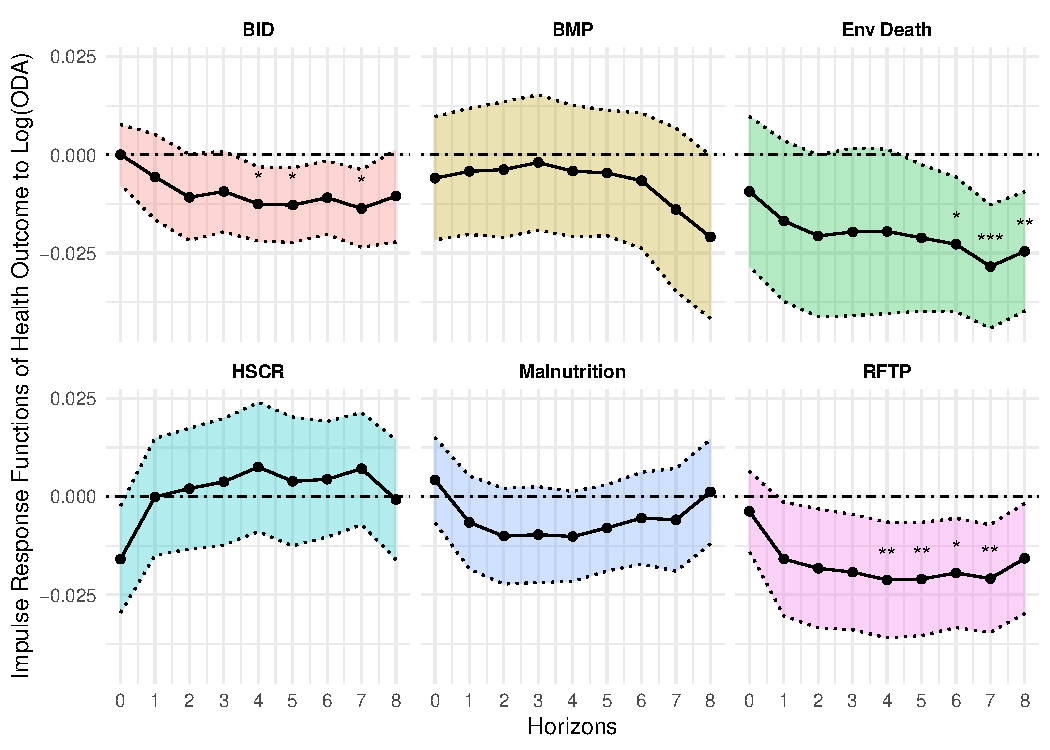
\includegraphics[width = 0.9\textwidth]{Results_outputs/Models/Local_Projt.pdf}
    \caption*{\footnotesize{Note: Author's computation. $^{*}$p$<$0.1; $^{**}$p$<$0.05; $^{***}$p$<$0.01}}
    \label{fig:Local_projection}
\end{figure}

As shown in Figure \ref{fig:Local_projection}, the local projection result is consistent with previously presented methods, showing the anticipated direction of effect for all health dimensions. Accordingly, contemporaneous ODA has positive impacts on the burden of infection and diseases (BID), environmental death, and reproductive fatalities (RFTP), though some effects are weaker than others. Specifically, ODA exhibits the strongest intermediate and long-term effects on reproductive fatalities, with the effect becoming statistically significant after five years (4th horizons) and lasting until the seventh year. While ODA is weakly significant for environmental death after six years (5th horizons), the significance level increases in the seventh and eighth years. Similarly, the impact of ODA on BID is weakly significant, starting from the fourth year and continuing until the seventh year. Surprisingly, ODA now shows positive impact on health system capacity and responsiveness starting from second horizon, albeit none is significant across the horizons. Also, ODA impact change direction on all health dimensions except mental burden, after the seventh year.    

\subsubsection*{\quad 5.2.2 Regional Heterogeneity of ODA Impact on Health Outcomes}
Similar to research question one, the thesis employs a combination of approaches: a unit fixed effect with time trend and FE-CLPM methods, to assess potential regional variations in the impact of ODA across health dimensions. The hypothesis is that:
 \begin{enumerate}[i]
    \item[ii] \textit{$H_0$: The impact of ODA on health is not significantly different between SSA and non-SSA regions on at least one health dimension.}
\end{enumerate} 
To test the hypothesis, the study employs the interaction of specific region dummy variables and one period lag of ODA to isolate the ODA impact in various regions. All models are estimated with five-period mean aggregated data like other models. The followings are the results:
\subsubsection*{\quad \quad \textit{5.2.2.1 Unit Fixed Model Model with Time Trend for Regional Heterogeneity:}}
\renewcommand{\arraystretch}{0.35} % 
\begin{longtable}{@{\extracolsep{-3pt}}lcccccc} 
\caption{Regional Heterogeneity: Unit FE Model with Time Trend}
\\[-0.9ex]\hline 
\hline \\[-0.9ex] 
 & \multicolumn{6}{c}{\textit{Dependent variables:}} \\ 
\cline{2-7} 
\\[-0.9ex] 
 & Reprod. & Infect. \& & Mental & Malnutr- & Envir.  & Health\\
& Fatality & Diseases & Burden & tion & Death & Capacity  \\
\\[-1.8ex] & (1) & (2) & (3) & (4) & (5) & (6)\\ 
\hline \\[-0.9ex]
log(EAP\_ODA)$_{t-1}$             & $0.013$        & $-0.007$       & $0.001$      & $-0.003$       & $0.001$        & $-0.001$      \\
                          & $(0.010)$      & $(0.006)$      & $(0.009)$    & $(0.008)$      & $(0.004)$      & $(0.004)$     \\
                          &&&&&&\\
log(SSA\_ODA)$_{t-1}$    & $-0.005$       & $-0.004$       & $-0.020$     & $0.021$        & $0.010$        & $0.006$       \\
                          & $(0.015)$      & $(0.017)$      & $(0.021)$    & $(0.017)$      & $(0.011)$      & $(0.013)$     \\
                          &&&&&&\\
log(MENA\_ODA)$_{t-1}$   & $-0.027^{*}$   & $0.032^{**}$   & $-0.011$     & $0.002$        & $0.019$        & $0.011$       \\
                          & $(0.012)$      & $(0.012)$      & $(0.018)$    & $(0.013)$      & $(0.016)$      & $(0.006)$     \\
                          &&&&&&\\
log(LAC\_ODA)$_{t-1}$    & $-0.004$       & $0.010$        & $-0.010$     & $-0.003$       & $-0.002$       & $-0.008$      \\
                          & $(0.014)$      & $(0.014)$      & $(0.010)$    & $(0.014)$      & $(0.014)$      & $(0.007)$     \\
                          &&&&&&\\
log(SCA\_ODA)$_{t-1}$    & $-0.022$       & $0.026$        & $0.003$      & $0.030$        & $0.000$        & $0.037$       \\
                          & $(0.036)$      & $(0.035)$      & $(0.043)$    & $(0.018)$      & $(0.041)$      & $(0.027)$     \\
                          &&&&&&\\
log(Europe\_ODA)$_{t-1}$ & $-0.032^{**}$  & $-0.009$       & $-0.016$     & $0.002$        & $-0.041^{*}$   & $-0.009$      \\
                          & $(0.011)$      & $(0.012)$      & $(0.013)$    & $(0.009)$      & $(0.017)$      & $(0.007)$     \\
\hline \\[-0.9ex]
Num.Obs. & \num{576} & \num{576} & \num{576} & \num{576} & \num{576} & \num{576}\\
R2 & \num{0.801} & \num{0.651} & \num{0.355} & \num{0.587} & \num{0.559} & \num{0.617}\\
R2 Adj. & \num{0.725} & \num{0.518} & \num{0.108} & \num{0.429} & \num{0.391} & \num{0.471}\\
AIC & \num{-1820.2} & \num{-1615.0} & \num{-1488.1} & \num{-1751.1} & \num{-1725.0} & \num{-1894.8}\\
BIC & \num{-1746.1} & \num{-1540.9} & \num{-1414.0} & \num{-1677.0} & \num{-1650.9} & \num{-1820.7}\\
RMSE & \num{0.05} & \num{0.06} & \num{0.06} & \num{0.05} & \num{0.05} & \num{0.05}\\
\bottomrule
\multicolumn{7}{l}{\scriptsize{$^{***}p<0.001$; $^{**}p<0.05$; $^{*}p<0.1$}}
\label{table:FE_RQ2}
\end{longtable}
According to the unit fixed effect model shown in Table \ref{table:FE_RQ2}, the impact of ODA weakly varies both across health dimensions and regions. While ODA shows the expected direction of effect on all health dimensions for SSA region except for malnutrition and environmental death, none is significant for the region. Notably, while ODA has positive and mildly significant impact at 5\% on reproductive fatality (RFTP) in the Middle East and North Africa (MENA), it increases burden of infection and diseases in the region. Moreover, ODA has weak significance (at 10\%) on environmental death and reproductive fatality (at 5\%) p\_value in Europe respectively. While the coefficient ODA is positive on health system capacity (HSCR) in SSA, MENA, SCA and Europe, it has negative effect on the dimension in EAP and LAC, albeit none is significant. Aside from these notable differences, the impact of ODA is not significantly different across regions on the rest of the health dimensions.


\subsubsection*{\quad \quad \textit{5.2.2.2 FE-CLDM for Regional Heterogeneity:}}
%list(RFTP_Region_DPM, BID_Region_dpm, BMP_Region_dpm, Malnuti_Region_dpm, EnvDeath_Region_dpm, HSCR_Region_dpm)
\renewcommand{\arraystretch}{0.35} % 
\begin{longtable}{@{\extracolsep{-3pt}}lcccccc} 
\caption{Regional Heterogeneity with FE-CLPM (linear-log model with aggregated data)} 
\\[-1ex]\hline 
\hline \\[-0.9ex] 
 & \multicolumn{6}{c}{\textit{Dependent variables:}} \\ 
\cline{2-7} 
\\[-0.9ex] 
 & Reprod. & Infect. \& & Mental & Malnutr- & Envir.  & Health\\
& Fatality & Diseases & Burden & tion & Death & Capacity  \\
\\[-1ex]
& (1) & (2) & (3) & (4) & (5) & (6)\\ 
\hline \\[-0.9ex]
log(EAP\_ODA)$_{t-1}$                   & $0.005$       & $-0.030$      & $-0.001$      & $-0.041$      & $0.004$       & $0.006$       \\
                                & $(0.011)$     & $(0.023)$     & $(0.024)$     & $(0.023)$     & $(0.018)$     & $(0.017)$     \\
                                &&&&&&\\
log(SSA\_ODA)$_{t-1}$                        & $-0.051$      & $-0.035$      & $-0.043$      & $0.096^{*}$   & $-0.030$      & $0.031$       \\
                                & $(0.030)$     & $(0.045)$     & $(0.053)$     & $(0.043)$     & $(0.040)$     & $(0.041)$     \\
                                &&&&&&\\
log(MENA\_ODA)$_{t-1}$                       & $-0.011$      & $0.061$       & $0.023$       & $0.037$       & $0.011$       & $-0.020$      \\
                                & $(0.020)$     & $(0.031)$     & $(0.039)$     & $(0.032)$     & $(0.036)$     & $(0.029)$     \\
                                &&&&&&\\
log(LAC\_ODA)$_{t-1}$                        & $0.192^{**}$  & $-0.217^{**}$ & $-0.422^{*}$  & $-0.213^{**}$ & $0.264^{**}$  & $-0.284^{**}$ \\
                                & $(0.067)$     & $(0.083)$     & $(0.188)$     & $(0.072)$     & $(0.086)$     & $(0.087)$     \\
                                &&&&&&\\
log(SCA\_ODA)$_{t-1}$                        & $-0.056$      & $-0.088$      & $-0.068$      & $0.239^{***}$ & $-0.008$      & $-0.102$      \\
                                & $(0.039)$     & $(0.068)$     & $(0.080)$     & $(0.067)$     & $(0.050)$     & $(0.064)$     \\
                                &&&&&&\\
log(Europe\_ODA)$_{t-1}$                     & $-0.037$      & $0.031$       & $-0.008$      & $0.058$       & $-0.068^{*}$  & $-0.005$      \\
                                & $(0.021)$     & $(0.029)$     & $(0.035)$     & $(0.032)$     & $(0.030)$     & $(0.029)$     \\
                                &&&&&&\\
%log\_ae                         & $0.037$       & $0.005$       & $-0.073$      & $0.015$       & $-0.032$      & $0.021$       \\
%                                & $(0.055)$     & $(0.059)$     & $(0.078)$     & $(0.049)$     & $(0.041)$     & $(0.055)$     \\
%log\_GDP\_Cap                   & $0.086$       & $-0.022$      & $0.037$       & $-0.052$      & $-0.022$      & $0.234^{***}$ \\
 %                               & $(0.047)$     & $(0.060)$  & $(0.060)$     & $(0.114)$     & $(0.060)$     & $(0.067)$     \\
%FDI                             & $-0.001$      & $-0.001$      & $-0.002$      & $-0.001$      & $-0.001$      & $0.000$       \\
 %                               & $(0.001)$     & $(0.001)$     & $(0.001)$     & $(0.002)$     & $(0.001)$     & $(0.001)$     \\
%log\_CRI\_Score                 & $0.001$       & $0.012$       & $-0.035$      & $-0.013$      & $0.065^{*}$   & $-0.052$      \\
 %                               & $(0.017)$     & $(0.036)$     & $(0.039)$     & $(0.026)$     & $(0.031)$     & $(0.041)$     \\
%log\_Trade                      & $0.013$       & $0.055$       & $0.133^{*}$   & $-0.032$      & $0.058$       & $0.006$       \\
 %                               & $(0.028)$     & $(0.044)$     & $(0.064)$     & $(0.045)$     & $(0.039)$     & $(0.042)$     \\
%log\_hlth\_Per\_Cap             & $0.020$       & $-0.037$      & $0.060$       & $0.016$       & $0.063$       & $0.110^{*}$   \\
%                                & $(0.026)$     & $(0.048)$     & $(0.056)$     & $(0.048)$     & $(0.042)$     & $(0.046)$     \\
%log\_gov                        & $-0.120$      & $0.110$       & $0.063$       & $-0.340^{**}$ & $-0.125$      & $0.156$       \\
 %                               & $(0.069)$     & $(0.083)$     & $(0.109)$     & $(0.110)$     & $(0.093)$     & $(0.093)$     \\
%log\_External\_debt             & $-0.006$      & $-0.022$      & $-0.059^{*}$  & $0.067^{**}$  & $-0.000$      & $-0.008$      \\
 %                               & $(0.016)$     & $(0.018)$     & $(0.024)$     & $(0.021)$     & $(0.018)$     & $(0.019)$     \\
%Autoregressive Parameter   & $0.770^{***}$ &     $0.953^{***}$          &    $0.987^{***}$           &    $0.829^{***}$           &     $0.737^{***}$          &        $0.783^{***}$       \\
 %                               & $(0.043)$     & $(0.093)$       % &   $(0.100)$             &       $(0.096)$        &       $(0.121)$        &    $(0.112)$           \\

Reprod\_Fatality$_{(t - 1)}$ &  $0.770^{***}$  &&&&&\\
&  $(0.043)$ & &&&&\\
&&&&&&\\
Infection\_Diseas$_{(t - 1)}$   &               & $0.953^{***}$ &               &               &               &               \\
                                &               & $(0.093)$     &               &               &               &               \\
&&&&&&\\
Mental\_Burden$_{(t - 1)}$   &               &               & $0.987^{***}$ &               &               &               \\
                                &               &               & $(0.100)$     &               &               &               \\
                                &&&&&&\\
Malnutrition$_{(t - 1)}$   &               &               &               & $0.829^{***}$ &               &               \\
                                &               &               &               & $(0.096)$     &               &               \\
&&&&&&\\
Environ\_Death$_{(t - 1)}$ &               &               &               &               & $0.737^{***}$ &               \\
                                &               &               &               &               & $(0.121)$     &               \\
                                &&&&&&\\
 HealthSys\_Capacity$_{(t - 1)}$     &               &               &               &               &               & $0.783^{***}$ \\
 %                               &               &               &               &               &               & $(0.112)$     \\
\hline \\[-0.9ex]
DF                              & $125.000$     & $125.000$     & $125.000$     & $125.000$     & $125.000$     & $125.000$     \\
Chi-square ($\chi^2$)                           & $280.205$     & $211.046$     & $233.490$     & $259.328$     & $184.373$     & $193.121$     \\
Observation (N)                               & $144.000$     & $144.000$     & $144.000$     & $144.000$     & $144.000$     & $144.000$     \\
RMSEA                           & $0.093$       & $0.069$       & $0.078$       & $0.086$       & $0.057$       & $0.062$       \\
RMSEA 90\% CI Lower                  & $0.078$       & $0.053$       & $0.062$       & $0.071$       & $0.039$       & $0.044$       \\
RMSEA 90\% CI Upper                  & $0.107$       & $0.085$       & $0.093$       & $0.101$       & $0.074$       & $0.078$       \\
p(RMSEA $<$ 0.05)                    & $0.000$       & $0.030$       & $0.003$       & $0.000$       & $0.238$       & $0.134$       \\
SRMR                            & $0.007$       & $0.011$       & $0.011$       & $0.008$       & $0.009$       & $0.009$       \\
\hline
%\multicolumn{7}{l}
%\scriptsize{$^{***}p<0.001$; $^{**}p<0.01$; $^{*}p<0.05$}}
%\end{tabular}
\caption*{\scriptsize{Note: Only the ODA coefficient are presented. ODA estimate represents the EAP region estimate, to avoid binary trap. $^{***}p<0.001$; $^{**}p<0.05$; $^{*}p<0.1$}}
\label{table:DPM_RQ2}
%\end{center}
\end{longtable}


Unlike the unit FE model, the FE-CLPM presented in Figure \ref{table:DPM_RQ2} shows a slightly different result. While the direction of effect is similar to FE model, ODA now has a weak significant effect on environmental death in SSA region. Moreover and surprisingly, the coefficients of ODA across all health dimensions are significant for Latin America and the Caribbean (LAC), albeit positive estimates for environmental death and negative for health system capacity. Due to result inconsistency, it is difficult to conclude that the impact of ODA significantly varies across the regions.  


%is mildly   reveals that the coefficient of the interaction between one-period-lagged ODA and the SSA dummy is statistically significant for infections and diseases. Specifically, a one percentage increase in ODA to the SSA region reduces infections and diseases by 0.075 standard deviations, with significance at the 5\% level, indicating a statistical difference between SSA countries and non-SSA countries. While the coefficients of ODA on other health dimensions show desired directions, except for malnutrition, they are not statistically significant.     

\subsubsection*{\quad 5.2.3 Mediation Path Analysis of Social Protection in ODA's Impact on Health}
\renewcommand{\arraystretch}{0.7} % 
% Table created by stargazer v.5.2.3 by Marek Hlavac, Social Policy Institute. E-mail: marek.hlavac at gmail.com
% Date and time: Tue, Dec 26, 2023 - 08:41:47
\begin{table}[!htbp] \centering 
  \caption{Mediation Analysis of Social Protection in the ODA's Impact on Health Dimensions} 
  \label{tab:MediationModel} 
\begin{tabular}{@{\extracolsep{-3pt}}lcccccc} 
\\[-1.8ex]\hline 
\hline \\[-1.8ex] 
 & \multicolumn{6}{c}{\textbf{Main Predictor: log(ODA)$_{it-4}$}} \\
 & & & & & & \\ 
 & \multicolumn{6}{c}{\textbf{Mediating Variable: Social\_Protection\_Coverage$_{it-3}$}} \\
\cline{2-7} 
\\[-1.8ex] & \multicolumn{6}{c}{ } \\ 
\textbf{Dependent} & Reproductive & Malnutrition  & Infections and & Health & Envir. & Mental\\
\textbf{Variables}: & Fatalities & & Diseases & Capacity & Death & Burden \\
\\[-1.8ex] & (1) & (2) & (3) & (4) & (5) & (6)\\ 
\hline \\[-1.8ex] 
\textbf{Total Effect}: & $-$0.008$^{***}$ & $-$0.015 &$-$0.002 & 0.031 & $-$0.006 & 0.026 \\
 & (0.002)& (0.020)& (0.002)& (0.025) & (0.015)& (0.016)\\
 & & & & & & \\ 
 \textbf{Direct Effect}: & $-$0.008$^{***}$ & $-$0.015 & $-$0.002 & 0.031 & $-$0.006 & 0.026\\
 & (0.002) & (0.020) & (0.002) & (0.025) & (0.015)&  (0.016)\\
 & & & & & & \\  
 \textbf{Indirect Effect}: & $-$0.000 & 0.000 & $-$0.000 & $-$0.000 & 0.000 & $-$0.000\\
 \textbf{Lower CI}: & $-$0.00010 &$-$0.00253 &  $-$0.00005 & $-$0.00245  &  $-$0.00217 & $-$0.00060\\ 
\textbf{Upper CI}: & 0.00006 & 0.00258 & 0.00004 & 0.00218 & 0.00249 & 0.000347 \\
 & & & & & & \\ 
\hline \\[-1.8ex] 
Level of & & & & & & \\
Confidence: & 95\% & 95\% & 95\% & 95\% & 95\% & 95\%\\
Bootstrap &&&&&& \\
Replicates: & 5000 & 5000 & 5000 & 5000 & 5000 & 5000\\
\bottomrule
\hline \\[-1.8ex] 
\textit{Note:}  & \multicolumn{6}{r}{$^{*}$p$<$0.1; $^{**}$p$<$0.05; $^{***}$p$<$0.01} \\ 
\end{tabular} 
\end{table} 



This section presents the result, in Table \ref{tab:MediationModel}, on the mediating role of social protection in the impact of ODA on various health dimensions.
The hypothesis is that:
 \begin{enumerate}[i]
    \item[iii] \textit{$H_0$: The indirect effect of social protection in the impact of ODA on health is not significant on at least one health dimension.}
\end{enumerate} 
For modelling convenience and in line with the causal order: \(ODA_{it-4} \rightarrow SP_{it-3} \rightarrow HO_{it}\) (see Chapter Three, Methodology, for details), year-wave data is employed in the analysis. All relevant variables were demeaned within to reflect the unit FE method, and respective lag and log transformations of relevant variables were performed before modeling. Additionally, a time trend variable was included like other models and the standard errors are corrected using robust error and the bootstrap procedure with 5000 replications across all health dimensions.

The mediation result, in Table \ref{tab:MediationModel}, shows that ODA has a highly significant and positive impact on reproductive fatalities (RFTP), with an average reduction of 0.008 standard deviations in response to a 1\% change in ODA. While ODA exhibits the desired direction of coefficients for other health dimensions, except mental health, they are statistically insignificant. Since the direct effect of all ODA on health remains the same as the total effect, and all confidence intervals of the indirect effect include zero, the result does not provide sufficient evidence that social protection has a significant mediating role in the effect of ODA on all health dimensions. It is important to note that the causal assumption used to derive the indirect effect assumes that treatment (ODA allocation) precedes the mediator (Social Protection), and the mediator, in turn, precedes the outcome (health). Any deviation from these assumptions, such as variations in lag periods, the direction of the relationship, or high missingness of social protection data, could imply potential underestimation or overestimation of the indirect effect. Therefore, this analysis serves as a simple policy guide for the optimal allocation of ODA to enhance health, recognizing its limitations.

\subsection*{5.3 Robustness Checks}
\addcontentsline{toc}{subsection}{5.3 Robustness Checks}
To assess the robustness of the findings presented above, the thesis estimated three models with two approaches. Unit FE with time trend as control and FE-CLDM are estimated for the overaching research question, while only the unit FE is employed for regional heterogeneity. Moreover, the main predictor is now social infrastructure ODA, as opposed to total ODA in the main models. All robustness models employ a similar set of covariates as the main models. Similar to the main models, these robustness models were implemented with aggregated data, and the results are presented in Table \ref{table:DPM_Robst_RQ1}, \ref{table:UnitFE_Robst_Region_RQ2}, and \ref{table:UnitFE_Robst_Region_RQ2}.
\subsubsection*{\quad 5.3.1 Robustness Checks: Impact of Social Infrastructure ODA on Health Outcomes}
\addcontentsline{toc}{subsubsection}{5.3.1 Impact of Social Infrastructure ODA on Health Outcomes}

%\subsection*{Appendix C.2: \quad Roburstness Models}
%\addcontentsline{toc}{subsection}{Appendix C.2: \quad Roburstness Models}
\renewcommand{\arraystretch}{0.35} % 
\begin{longtable}{@{\extracolsep{-3pt}}lcccccc} 
\caption{Robustness Unit FE Model with Social Infrastructure ODA} 
\\[-0.9ex]\hline 
\hline \\[-0.9ex] 
 & \multicolumn{6}{c}{\textit{Dependent variables:}} \\ 
\cline{2-7} 
\\[-0.9ex] 
 & Reprod. & Infect. \& & Mental & Malnutr- & Envir.  & Health\\
& Fatality & Diseases & Burden & tion & Death & Capacity  \\
\\[-1.8ex] & (1) & (2) & (3) & (4) & (5) & (6)\\ 
\hline \\[-0.9ex]
log(SocInfr\_ODA)$_{t-1}$ & $-0.008$       & $-0.027^{**}$  & $0.000$       & $0.015$        & $-0.025$       & $-0.023$      \\
                     & $(0.011)$      & $(0.010)$      & $(0.014)$     & $(0.014)$      & $(0.013)$      & $(0.013)$     \\
                     &&&&&&\\
Elect\_Access                   & $-0.007^{***}$ & $-0.005^{**}$  & $-0.003$      & $-0.003$       & $-0.001$       & $0.005^{***}$ \\
                     & $(0.002)$      & $(0.002)$      & $(0.002)$     & $(0.002)$      & $(0.001)$      & $(0.001)$     \\
                     &&&&&&\\
log(GDP\_PerCap)        & $-0.056$       & $-0.115^{*}$   & $0.032$       & $-0.494^{***}$ & $-0.227^{***}$ & $0.340^{***}$ \\
                     & $(0.083)$      & $(0.053)$      & $(0.075)$     & $(0.108)$      & $(0.066)$      & $(0.057)$     \\
                     &&&&&&\\
Climate\_Risk\_Index           & $0.001$        & $0.000$        & $0.001$       & $0.000$        & $0.001$        & $-0.001^{**}$ \\
                     & $(0.000)$      & $(0.000)$      & $(0.001)$     & $(0.001)$      & $(0.000)$      & $(0.000)$     \\
                     &&&&&&\\
log(Remittance)      & $-0.003$       & $0.002$        & $-0.002$      & $-0.005$       & $-0.004$       & $0.007$       \\
                     & $(0.003)$      & $(0.002)$      & $(0.003)$     & $(0.006)$      & $(0.003)$      & $(0.004)$     \\
                     &&&&&&\\
log(Population)             & $-1.053^{***}$ & $-0.859^{***}$ & $-0.093$      & $-0.645^{*}$   & $-0.065$       & $-0.209$      \\
                     & $(0.311)$      & $(0.223)$      & $(0.524)$     & $(0.295)$      & $(0.407)$      & $(0.194)$     \\
                     &&&&&&\\
log(Pop\_Density)       & $0.313$        & $0.434^{*}$    & $0.189$       & $-0.088$       & $-0.133$       & $0.454^{**}$  \\
                     & $(0.229)$      & $(0.207)$      & $(0.508)$     & $(0.231)$      & $(0.358)$      & $(0.148)$     \\
                     &&&&&&\\
log(Hlth\_Spnd\_PerCap)  & $0.044$        & $0.038$        & $0.106^{*}$   & $-0.075$       & $0.086$        & $0.083^{*}$   \\
                     & $(0.048)$      & $(0.044)$      & $(0.047)$     & $(0.070)$      & $(0.053)$      & $(0.037)$     \\
                     &&&&&&\\
Governance\_Index                  & $-0.044$       & $-0.017$       & $-0.025$      & $-0.166^{***}$ & $-0.063$       & $0.076$       \\
                     & $(0.046)$      & $(0.043)$      & $(0.053)$     & $(0.049)$      & $(0.049)$      & $(0.048)$     \\
                     &&&&&&\\
log(External\_Debt)  & $0.025$        & $0.006$        & $0.006$       & $0.033$        & $-0.023$       & $-0.033^{*}$  \\
                     & $(0.018)$      & $(0.015)$      & $(0.015)$     & $(0.018)$      & $(0.018)$      & $(0.016)$     \\
                     &&&&&&\\
Time\_Trend            & $-0.046^{***}$ & $-0.023^{**}$  & $-0.054^{**}$ & $0.008$        & $-0.063^{***}$ & $0.018$       \\
                     & $(0.011)$      & $(0.009)$      & $(0.017)$     & $(0.013)$      & $(0.016)$      & $(0.011)$     \\
\hline[-0.9ex]
Num.Obs. & \num{576} & \num{576} & \num{576} & \num{576} & \num{576} & \num{576}\\
R2 & \num{0.765} & \num{0.573} & \num{0.251} & \num{0.622} & \num{0.562} & \num{0.583}\\
R2 Adj. & \num{0.678} & \num{0.416} & \num{-0.024} & \num{0.484} & \num{0.401} & \num{0.430}\\
AIC & \num{-1154.3} & \num{-1248.9} & \num{-866.7} & \num{-1007.1} & \num{-1003.5} & \num{-1026.4}\\
BIC & \num{-1102.0} & \num{-1196.6} & \num{-814.4} & \num{-954.8} & \num{-951.2} & \num{-974.1}\\
RMSE & \num{0.09} & \num{0.08} & \num{0.11} & \num{0.10} & \num{0.10} & \num{0.10}\\
\bottomrule
\multicolumn{7}{l}{\scriptsize{$^{***}p<0.001$; $^{**}p<0.05$; $^{*}p<0.1$}}
\label{table:UnitFE_Robst_RQ1}
\end{longtable}

Accordingly, the unit FE model in Table \ref{table:UnitFE_Robst_Region_RQ2}, shows that social infrastructure ODA has positive impact across various health dimensions except malnutrition and health system capacity, albeit insignificant. Moreover, unlike the total ODA, the coefficient of social infrastructure ODA has a positive and mildly significant impact on burden of infection and diseases (BID) with the coefficient value of - 0.027 standard deviations. 
\renewcommand{\arraystretch}{0.35} % 
\begin{longtable}{@{\extracolsep{-3pt}}lcccccc} 
\caption{Robustness FE-CLPM Model with Social Infrastructure ODA} 
\\[-1.8ex]\hline 
\hline \\[-0.9ex] 
 & \multicolumn{6}{c}{\textit{Dependent variables:}} \\ 
\cline{2-7} 
\\[-0.9ex] 
 & Reprod. & Infect. \& & Mental & Malnutr- & Envir.  & Health\\
& Fatality & Diseases & Burden & tion & Death & Capacity  \\
\\[-1.8ex] & (1) & (2) & (3) & (4) & (5) & (6)\\ 
\hline \\[-0.9ex]
log(SocInfr\_ODA)$_{t-1}$            & $-0.065^{***}$ & $-0.077^{***}$ & $-0.137$      & $-0.096^{***}$ & $-0.094^{***}$ & $-0.130^{***}$ \\
                                & $(0.013)$      & $(0.016)$      & $(0.073)$     & $(0.024)$      & $(0.018)$      & $(0.026)$      \\
                                &&&&&&\\
Elect\_Access                              & $0.000$        & $-0.001$       & $-0.001$      & $0.001$        & $0.001$        & $0.003^{*}$    \\
                                & $(0.001)$      & $(0.001)$      & $(0.002)$     & $(0.001)$      & $(0.001)$      & $(0.001)$      \\
                                &&&&&&\\
log(GDP\_PerCap)p                   & $0.053$        & $-0.014$       & $0.073$       & $-0.034$       & $0.010$        & $0.188^{**}$   \\
                                & $(0.037)$      & $(0.069)$      & $(0.070)$     & $(0.096)$      & $(0.052)$      & $(0.069)$      \\
                                &&&&&&\\
log(Remittance)                 & $0.001$        & $0.003$        & $0.008$       & $-0.004$       & $0.003$        & $0.005$        \\
                                & $(0.002)$      & $(0.003)$      & $(0.004)$     & $(0.002)$      & $(0.002)$      & $(0.003)$      \\
                                &&&&&&\\
Climate\_Risk\_Index                      & $-0.000$       & $-0.000$       & $-0.001$      & $-0.001$       & $0.001$        & $-0.001$       \\
                                & $(0.000)$      & $(0.000)$      & $(0.001)$     & $(0.000)$      & $(0.000)$      & $(0.001)$      \\
                                &&&&&&\\
log(Hlth\_Spnd\_PerCap)             & $0.014$        & $-0.050$       & $0.008$       & $0.026$        & $0.099^{*}$    & $0.125^{**}$   \\
                                & $(0.022)$      & $(0.044)$      & $(0.057)$     & $(0.058)$      & $(0.042)$      & $(0.044)$      \\
                                &&&&&&\\
 Governance\_Index                            & $-0.036$       & $0.013$        & $0.027$       & $-0.064$       & $-0.032$       & $0.029$        \\
                                & $(0.028)$      & $(0.036)$      & $(0.069)$     & $(0.042)$      & $(0.043)$      & $(0.041)$      \\
                                &&&&&&\\
log(External\_Debt)             & $0.011$        & $-0.009$       & $-0.056^{**}$ & $0.048^{*}$    & $0.011$        & $-0.003$       \\
                                & $(0.016)$      & $(0.016)$      & $(0.021)$     & $(0.020)$      & $(0.017)$      & $(0.016)$      \\
                                &&&&&&\\
Reprod\_Fatality$_{(t - 1)}$    & $0.760^{***}$  &                &               &                &                &                \\
                                & $(0.036)$      &                &               &                &                &                \\
                                &&&&&&\\
Infection\_Diseas$_{(t - 1)}$   &                & $1.082^{***}$  &               &                &                &                \\
                                &                & $(0.062)$      &               &                &                &                \\
                                &&&&&&\\
Mental\_Burden$_{(t - 1)}$   &                &                & $1.220^{***}$ &                &                &                \\
                                &                &                & $(0.075)$     &                &                &                \\
                                &&&&&&\\
Malnutrition$_{(t - 1)}$   &                &                &               & $0.814^{***}$  &                &                \\
                                &                &                &               & $(0.087)$      &                &                \\
                                &&&&&&\\
Environ\_Death$_{(t - 1)}$  &                &                &               &                & $0.812^{***}$  &                \\
                                &                &                &               &                & $(0.089)$      &                \\
                                &&&&&&\\
HealthSys\_Capacity$_{(t - 1)}$     &                &                &               &                &                & $0.882^{***}$  \\
                                &                &                &               &                &                & $(0.092)$      \\
                                
\hline \\[-0.9ex]
DF                              & $89.000$       & $89.000$       & $89.000$      & $89.000$       & $89.000$       & $89.000$       \\
Chi-square ($\chi^2$)                           & $264.295$      & $212.761$      & $238.637$     & $280.669$      & $150.289$      & $161.800$      \\
Observation (N)                               & $144.000$      & $144.000$      & $144.000$     & $144.000$      & $144.000$      & $144.000$      \\
RMSEA                           & $0.117$        & $0.098$        & $0.108$       & $0.122$        & $0.069$        & $0.075$        \\
RMSEA 90\% CI Lower                  & $0.101$        & $0.081$        & $0.092$       & $0.106$        & $0.049$        & $0.057$        \\
RMSEA 90\% CI Upper                  & $0.133$        & $0.115$        & $0.125$       & $0.139$        & $0.088$        & $0.094$        \\
rmsea.pvalue                    & $0.000$        & $0.000$        & $0.000$       & $0.000$        & $0.054$        & $0.015$        \\
srmr                            & $0.009$        & $0.018$        & $0.020$       & $0.013$        & $0.010$        & $0.009$        \\
\hline
\multicolumn{7}{l}{\scriptsize{$^{***}p<0.001$; $^{**}p<0.05$; $^{*}p<0.1$}}
\label{table:DPM_Robst_RQ1}
\end{longtable}


Similar to the FE-CLPM in the main model, the robustness FE-CLPM model  in Table \ref{table:DPM_Robst_RQ1} shows strong positive and significant impact of social infrastructure ODA for all health dimensions, except the burden of mental problem (BMP) and health system capacity. While the result is consistent with the main models, malnutrition are now strongly significant. Surprisingly, the coefficient of social infrastructure ODA is highly significant and negative for health system capacity, indicating that both social infrastructure and total ODA has exert negative impact on countries health system capacity. Till this end, there is evidence that total and social infrastructure ODA have significant positive impact on reproductive fatality (RFTP), burden of infection and diseases (BID), malnutrition and environmental death. 

\subsubsection*{\quad 5.3.2 Robustness Checks: Regional Variation of Social Infrastructure ODA's Impact}
\addcontentsline{toc}{subsubsection}{5.3.2 Regional Variation of Social Infrastructure ODA's Impact}

Unlike the main regional model, the social infrastructure ODA, as shown the unit FE model in Table \ref{table:UnitFE_Robst_Region_RQ2}, has no significant variation among the regions compared. Specifically, while social infrastructure ODA shows the expected impact on all health dimensions for SSA, except burden of mental problem, none is significant. Similar pattern of result of observed across other regions. Notably,social infrastructure ODA has most negative impact on health system capacity in East Asia and Pacific (EAP) and  Middle East and North Africa (MENA) region, though none is significant.  
\renewcommand{\arraystretch}{0.35} % 
 \begin{longtable}{@{\extracolsep{-3pt}}lcccccc} 
\caption{Robustness Regional Variation with Unit FE for Social Infrastructure ODA} 
\\[-0.9ex]\hline 
\hline \\[-0.9ex] 
 & \multicolumn{6}{c}{\textit{Dependent variables:}} \\ 
\cline{2-7} 
\\[-0.9ex] 
 & Reprod. & Infect. \& & Mental & Malnutr- & Envir.  & Health\\
& Fatality & Diseases & Burden & tion & Death & Capacity  \\
\\[-0.9ex] & (1) & (2) & (3) & (4) & (5) & (6)\\ 
\hline \\[-0.9ex]
log(EAP\_SocInfr\_ODA)$_{t-1}$  & $0.022$        & $-0.002$       & $0.010$       & $-0.003$       & $0.003$        & $-0.014$      \\
                      & $(0.028)$      & $(0.016)$      & $(0.016)$     & $(0.020)$      & $(0.015)$      & $(0.016)$     \\
                      &&&&&&\\
log(SSA\_SocInfr\_ODA)$_{t-1}$      & $-0.017$       & $-0.008$       & $-0.020$      & $0.007$        & $-0.016$       & $0.010$       \\
                      & $(0.031)$      & $(0.024)$      & $(0.022)$     & $(0.026)$      & $(0.016)$      & $(0.021)$     \\
                      &&&&&&\\
log(MENA\_SocInfr\_ODA)$_{t-1}$     & $-0.017$       & $0.002$        & $0.047$       & $0.045$        & $-0.028$       & $-0.004$      \\
                      & $(0.030)$      & $(0.024)$      & $(0.035)$     & $(0.027)$      & $(0.029)$      & $(0.018)$     \\
                      &&&&&&\\
log(LAC\_SocInfr\_ODA)$_{t-1}$      & $-0.034$       & $-0.030$       & $-0.014$      & $0.014$        & $-0.005$       & $0.011$       \\
                      & $(0.032)$      & $(0.018)$      & $(0.018)$     & $(0.023)$      & $(0.021)$      & $(0.018)$     \\
                      &&&&&&\\
log(SCA\_SocInfr\_ODA)$_{t-1}$    & $0.030$        & $0.037$        & $0.006$       & $0.038$        & $0.025$        & $0.038$       \\
                      & $(0.045)$      & $(0.028)$      & $(0.044)$     & $(0.026)$      & $(0.029)$      & $(0.023)$     \\
                      &&&&&&\\
log(Europe\_SocInfr\_ODA)$_{t-1}$ & $-0.054$       & $0.028$        & $-0.039$      & $-0.023$       & $-0.025$       & $0.031$       \\
                      & $(0.037)$      & $(0.054)$      & $(0.060)$     & $(0.031)$      & $(0.071)$      & $(0.019)$     \\
                      &&&&&&\\
Elect\_Access                    & $-0.002^{**}$  & $-0.002^{*}$   & $-0.002$      & $-0.000$       & $0.000$        & $0.003^{***}$ \\
                      & $(0.001)$      & $(0.001)$      & $(0.001)$     & $(0.001)$      & $(0.001)$      & $(0.001)$     \\
                      &&&&&&\\
log(GDP\_PerCap)         & $-0.088$       & $-0.149^{***}$ & $-0.018$      & $-0.284^{***}$ & $-0.102^{**}$  & $0.147^{***}$ \\
                      & $(0.047)$      & $(0.033)$      & $(0.044)$     & $(0.049)$      & $(0.034)$      & $(0.032)$     \\
                      &&&&&&\\
Climate\_Risk\_Index            & $0.000$        & $0.000$        & $0.000$       & $0.000$        & $0.000$        & $-0.001^{*}$  \\
                      & $(0.000)$      & $(0.000)$      & $(0.000)$     & $(0.000)$      & $(0.000)$      & $(0.000)$     \\
                      &&&&&&\\
log(Remittance)       & $-0.001$       & $0.002$        & $-0.002$      & $-0.002$       & $-0.002$       & $0.003$       \\
                      & $(0.001)$      & $(0.002)$      & $(0.002)$     & $(0.003)$      & $(0.002)$      & $(0.002)$     \\
                      &&&&&&\\
log(Population)              & $-0.612$       & $-0.569^{***}$ & $-0.292$      & $-0.127$       & $-0.118$       & $0.149$       \\
                      & $(0.413)$      & $(0.155)$      & $(0.255)$     & $(0.171)$      & $(0.328)$      & $(0.103)$     \\
                      &&&&&&\\
log(Pop\_Density)        & $0.542$        & $0.226$        & $0.140$       & $-0.119$       & $0.135$        & $0.086$       \\
                      & $(0.408)$      & $(0.118)$      & $(0.243)$     & $(0.142)$      & $(0.310)$      & $(0.070)$     \\
                      &&&&&&\\
log(Hlth\_Spnd\_PerCap)   & $-0.001$       & $-0.016$       & $0.073^{*}$   & $-0.063$       & $0.003$        & $0.019$       \\
                      & $(0.025)$      & $(0.031)$      & $(0.035)$     & $(0.040)$      & $(0.027)$      & $(0.019)$     \\
                      &&&&&&\\
Governance\_Index                   & $-0.051$       & $-0.063^{*}$   & $-0.013$      & $-0.077^{**}$  & $-0.042$       & $0.037$       \\
                      & $(0.030)$      & $(0.027)$      & $(0.031)$     & $(0.025)$      & $(0.026)$      & $(0.023)$     \\
                      &&&&&&\\
log(External\_Debt)   & $-0.006$       & $0.013$        & $0.007$       & $0.006$        & $-0.010$       & $-0.019^{*}$  \\
                      & $(0.008)$      & $(0.011)$      & $(0.010)$     & $(0.011)$      & $(0.010)$      & $(0.008)$     \\
                      &&&&&&\\
Time\_Trend             & $-0.065^{***}$ & $-0.026^{***}$ & $-0.023^{**}$ & $-0.003$       & $-0.043^{***}$ & $0.001$       \\
                      & $(0.007)$      & $(0.008)$      & $(0.008)$     & $(0.007)$      & $(0.010)$      & $(0.004)$     \\
\hline \\[-0.9ex]
Num.Obs. & \num{576} & \num{576} & \num{576} & \num{576} & \num{576} & \num{576}\\
R2 & \num{0.800} & \num{0.649} & \num{0.359} & \num{0.595} & \num{0.523} & \num{0.612}\\
R2 Adj. & \num{0.724} & \num{0.515} & \num{0.114} & \num{0.440} & \num{0.341} & \num{0.464}\\
AIC & \num{-1816.7} & \num{-1611.7} & \num{-1492.0} & \num{-1762.1} & \num{-1679.7} & \num{-1887.3}\\
BIC & \num{-1742.6} & \num{-1537.7} & \num{-1417.9} & \num{-1688.0} & \num{-1605.6} & \num{-1813.2}\\
RMSE & \num{0.05} & \num{0.06} & \num{0.06} & \num{0.05} & \num{0.05} & \num{0.05}\\
\bottomrule
\multicolumn{7}{l}{\scriptsize{$^{***}p<0.001$; $^{**}p<0.05$; $^{*}p<0.1$}}
\label{table:UnitFE_Robst_Region_RQ2}
\end{longtable}


%log(SocInfr\_ODA)$_{t-1}$ Elect\_Access log(GDP\_PerCap) Climate\_Risk\_Index log(Remittance) log(Population) log(Pop\_Density) log(Hlth\_Spnd\_PerCap) Governance\_Index log(External\_Debt) Time\_Trend  Reprod\_Fatality$_{(t - 1)}$  Infection\_Diseas$_{(t - 1)}$ Mental\_Burden$_{(t - 1)}$ Malnutrition$_{(t - 1)}$  Environ\_Death$_{(t - 1)}$ HealthSys\_Capacity$_{(t - 1)}$
The FE-CLDM model, on the other hand in Table \ref{table:DPM_Robst_Region_RQ2}, shows more complex result. Accordingly, social infrastructure ODA is found on reproductive fatality, infection and disease and HSCR for EAP, SSA, and MENA regions, all significant at 5\% p\_value. Notably, social infrastructure ODA impact on was also significant on malnutrition for EAP and SSA regions. A possible explanation for these sporadic significance results is that the social infrastructure ODA data employed is commitment, as opposed to disbursement data for total ODA in the main model. Due to inconsistency in results across the regional models and its complexity, the study do not have a conclusive evidence that the impact ODA varies between SSA and non-SSA regions.    

\renewcommand{\arraystretch}{0.35} % 
\begin{longtable}{@{\extracolsep{-3pt}}lccccc} 
\caption{Robustness Regional Variation with FE-CLPM Model for Social Infrastructure ODA} 
\\[-0.9ex]\hline 
\hline \\[-0.9ex] 
 & \multicolumn{5}{c}{\textit{Dependent variables:}} \\ 
\cline{2-6} 
\\[-0.9ex] 
 & Reprod. & Infect. \&  & Malnutr- & Envir.  & Health\\
& Fatality & Diseases & tion & Death & Capacity  \\
\\[-1.8ex] & (1) & (2) & (3) & (4) & (5)\\ 
\hline \\[-0.9ex]
log(EAP\_SocInfr\_ODA)$_{t-1}$            & $-0.111^{**}$ & $-0.087^{*}$  & $-0.150^{*}$  & $-0.049$      & $0.181^{**}$   \\
                                & $(0.036)$     & $(0.044)$     & $(0.074)$     & $(0.035)$     & $(0.066)$      \\
                                &&&&&\\
log(SSA\_SocInfr\_ODA)$_{t-1}$                & $0.128^{**}$  & $-0.054$      & $0.285^{**}$  & $-0.026$      & $-0.276^{**}$  \\
                                & $(0.04 0)$     & $(0.055)$     & $(0.087)$     & $(0.052)$     & $(0.086)$      \\
                                &&&&&\\
log(MENA\_SocInfr\_ODA)$_{t-1}$               & $0.131^{**}$  & $0.072$       & $0.076$       & $-0.003$      & $-0.189^{*}$   \\
                                & $(0.042)$     & $(0.051)$     & $(0.079)$     & $(0.049)$     & $(0.074)$      \\
                                &&&&&\\
log(LAC\_SocInfr\_ODA)$_{t-1}$                & $0.053$       & $0.003$       & $0.092$       & $-0.032$      & $-0.266^{***}$ \\
                                & $(0.041)$     & $(0.050)$     & $(0.077)$     & $(0.042)$     & $(0.074)$      \\
                                &&&&&\\
log(SCA\_SocInfr\_ODA)$_{t-1}$              & $-0.035$      & $0.085$       & $0.193^{*}$   & $0.118$       & $-0.282^{**}$  \\
                                & $(0.058)$     & $(0.066)$     & $(0.086)$     & $(0.072)$     & $(0.107)$      \\
                                &&&&&\\
log(Europe\_SocInfr\_ODA)$_{t-1}$           & $-0.078$      & $-0.140$      & $0.263$       & $-0.355^{*}$  & $-0.499^{**}$  \\
                                & $(0.093)$     & $(0.119)$     & $(0.140)$     & $(0.158)$     & $(0.163)$      \\
                                &&&&&\\
%log(Elect\_Access)                         & $0.063$       & $0.031$       & $0.031$       & $-0.002$      & $0.067$        \\
%                                & $(0.051)$     & $(0.068)$     & $(0.041)$     & $(0.040)$     & $(0.045)$      \\

%log(GDP\_PerCap)                   & $0.065$       & $0.015$       & $-0.045$      & $0.014$       & $0.182^{**}$   \\
  %                              & $(0.046)$     & $(0.072)$     & $(0.124)$     & $(0.054)$     & $(0.062)$      \\

%log(Hlth\_Spnd\_PerCap)             & $0.018$       & $-0.027$      & $0.001$       & $0.095^{*}$   & $0.128^{**}$   \\
 %                               & $(0.022)$     & $(0.045)$     & $(0.057)$     & $(0.042)$     & $(0.044)$      \\
%FDI                             & $-0.001$      & $0.000$       & $-0.001$      & $-0.000$      & $0.001$        \\
 %                               & $(0.001)$     & $(0.001)$     & $(0.002)$     & $(0.001)$     & $(0.001)$      \\
%Climate\_Risk\_Index                 & $-0.019$      & $0.014$       & $-0.017$      & $0.039$       & $-0.069$       \\
 %                               & $(0.016)$     & $(0.038)$     & $(0.025)$     & $(0.026)$     & $(0.040)$      \\
%log(Trade)                      & $0.039$       & $-0.008$      & $-0.012$      & $0.026$       & $-0.036$       \\
 %                               & $(0.031)$     & $(0.040)$     & $(0.052)$     & $(0.032)$     & $(0.047)$      \\
%log(Governance\_Index)                        & $-0.098$      & $0.004$       & $-0.223$      & $-0.106$      & $0.140$        \\
 %                               & $(0.066)$     & $(0.081)$     & $(0.125)$     & $(0.070)$     & $(0.092)$      \\
%log(External\_Debt)             & $-0.007$      & $-0.002$      & $0.039^{*}$   & $0.012$       & $-0.006$       \\
 %                               & $(0.014)$     & $(0.018)$     & $(0.020)$     & $(0.017)$     & $(0.019)$      \\
Reprod\_Fatality$_{(t - 1)}$    & $0.781^{***}$ &               &               &               &                \\
                                & $(0.042)$     &               &               &               &                \\
                                &&&&&\\
Infection\_Diseas$_{(t - 1)}$   &               & $1.018^{***}$ &               &               &                \\
                                &               & $(0.064)$     &               &               &                \\
                                &&&&&\\
Mental\_Burden$_{(t - 1)}$  &               &               & $0.808^{***}$ &               &                \\
                                &               &               & $(0.095)$     &               &                \\
                                &&&&&\\
Malnutrition$_{(t - 1)}$ &               &               &               & $0.749^{***}$ &                \\
                                &               &               &               & $(0.089)$     &                \\
                                &&&&&\\
HealthSys\_Capacity$_{(t - 1)}$    &               &               &               &               & $0.786^{***}$  \\
                                &               &               &               &               & $(0.091)$      \\
\hline \\[-0.9ex]
DF                              & $125.000$     & $125.000$     & $125.000$     & $125.000$     & $125.000$      \\
Chi-square ($\chi^2$)                          & $310.725$     & $266.087$     & $294.130$     & $218.675$     & $185.185$      \\
Observation (N)                               & $144.000$     & $144.000$     & $144.000$     & $144.000$     & $144.000$      \\
RMSEA                           & $0.102$       & $0.089$       & $0.097$       & $0.072$       & $0.058$        \\
RMSEA 90\% CI Lower                  & $0.087$       & $0.074$       & $0.083$       & $0.056$       & $0.039$        \\
RMSEA 90\% CI Upper                  & $0.116$       & $0.103$       & $0.111$       & $0.088$       & $0.075$        \\
p(RMSEA $<$ 0.05)                    & $0.000$       & $0.000$       & $0.000$       & $0.014$       & $0.226$        \\
SRMR                            & $0.006$       & $0.012$       & $0.004$       & $0.006$       & $0.005$        \\
\hline
\multicolumn{6}{l}{\scriptsize{$^{***}p<0.001$; $^{**}p<0.05$; $^{*}p<0.1$}}
\label{table:DPM_Robst_Region_RQ2}
\end{longtable}

      %Environ\_Death$_{(t - 1)}$ 

%the direction of the effect remains consistent with the main fixed effect model using total ODA, Social Infrastructure ODA exhibits significant impacts, particularly demonstrating the strongest effect on infections and diseases, and a weak effect on environmental death, and even an unexpected negative effect on health system capacity. Specifically, Social Infrastructure ODA, on average, reduces infections and diseases by 0.036 standard deviations and is highly significant. Moreover, environmental death is similarly impacted by Social Infrastructure ODA, with coefficients of -0.030, significant at a 5\% p-value. This result aligns with the GMM model presented in Table \ref{table:GMM_table}. While the direction of the effect for reproductive fatalities aligns with expectations, it is statistically insignificant, and health system capacity surprisingly exhibits a negative effect and is weakly significant.
%\renewcommand{\arraystretch}{0.85} % 

% Table created by stargazer v.5.2.3 by Marek Hlavac, Social Policy Institute. E-mail: marek.hlavac at gmail.com
% Date and time: Tue, Dec 26, 2023 - 09:18:33
\begin{table}[!htbp] \centering 
  \caption{Roburstness Check of Regional Variation with Social Infrastructure ODA} 
  \label{Tab:Robust_FE_RegHet} 
\begin{tabular}{@{\extracolsep{-2pt}}lcccccc} 
\\[-1.8ex]\hline 
\hline \\[-1.8ex] 
& \multicolumn{6}{c}{\textit{Dependent Variables:}} \\ 
\cline{2-7} 
\\[-1.8ex] & \multicolumn{6}{c}{ } \\ 
 & Reprod. & Malnutr-  & Infect. \& & Health & Envir. & Mental\\
 & Fatalities & ition & Diseases & Capacity & Death & Burden \\
 
\\[-1.8ex] & (1) & (2) & (3) & (4) & (5) & (6)\\ 
\hline \\[-1.8ex] 
  log(SOC\_INF\_ODA)$_{t-1}$ & $-$0.024$^{*}$ & 0.007 & $-$0.027$^{***}$ & $-$0.027$^{*}$ & $-$0.029$^{*}$ & 0.020 \\ 
  & (0.013) & (0.016) & (0.009) & (0.016) & (0.016) & (0.018) \\ 
  & & & & & & \\ 
 log(SOC\_INF\_ODA)$_{t-1}\times$SSA & 0.015 & 0.002 & $-$0.037 & 0.018 & $-$0.006 & $-$0.034 \\ 
  & (0.050) & (0.048) & (0.039) & (0.031) & (0.031) & (0.041) \\ 
  & & & & & & \\ 
log(Govt\_Hth\_Spnd) & $-$0.065 & $-$0.053 & $-$0.020 & 0.084$^{**}$ & $-$0.027 & 0.093$^{***}$ \\ 
  & (0.053) & (0.040) & (0.034) & (0.033) & (0.032) & (0.034) \\ 
  & & & & & & \\ 
 log(GDP\_per\_cap) & $-$0.162$^{**}$ & $-$0.239$^{***}$ & $-$0.183$^{***}$ & 0.196$^{***}$ & $-$0.308$^{***}$ & $-$0.054 \\ 
  & (0.081) & (0.073) & (0.056) & (0.058) & (0.053) & (0.063) \\ 
  & & & & & & \\ 
 log(Pop\_tot) & 0.024$^{***}$ & 0.034$^{***}$ & $-$0.015$^{*}$ & $-$0.018$^{***}$ & 0.024$^{**}$ & $-$0.021$^{*}$ \\ 
  & (0.008) & (0.009) & (0.008) & (0.007) & (0.010) & (0.012) \\ 
  & & & & & & \\ 
 Electricity\_access & $-$0.012$^{***}$ & $-$0.006$^{***}$ & $-$0.007$^{***}$ & 0.008$^{***}$ & $-$0.004$^{***}$ & $-$0.001 \\ 
  & (0.002) & (0.001) & (0.002) & (0.001) & (0.001) & (0.002) \\ 
  & & & & & & \\ 
 log(External\_debt) & 0.049$^{**}$ & 0.048$^{***}$ & 0.009 & $-$0.053$^{***}$ & $-$0.022 & 0.008 \\ 
  & (0.021) & (0.018) & (0.015) & (0.013) & (0.016) & (0.016) \\ 
  & & & & & & \\ 
 log(Trade) & $-$0.053 & 0.048 & 0.032 & $-$0.034 & 0.023 & 0.003 \\ 
  & (0.067) & (0.063) & (0.041) & (0.044) & (0.045) & (0.046) \\ 
  & & & & & & \\ 
 CRI\_score & 0.001$^{**}$ & 0.0003 & 0.001 & $-$0.001$^{***}$ & 0.001$^{*}$ & 0.001 \\ 
  & (0.001) & (0.001) & (0.0004) & (0.0004) & (0.0004) & (0.001) \\ 
  & & & & & & \\ 
 Governance & $-$0.049 & $-$0.220$^{***}$ & 0.025 & 0.081 & $-$0.044 & $-$0.039 \\ 
  & (0.058) & (0.055) & (0.044) & (0.065) & (0.051) & (0.058) \\ 
  & & & & & & \\ 
 FDI & $-$0.002 & $-$0.003$^{*}$ & $-$0.001 & 0.002$^{*}$ & $-$0.0003 & $-$0.0003 \\ 
  & (0.001) & (0.001) & (0.001) & (0.001) & (0.001) & (0.001) \\ 
  & & & & & & \\ 
 log(Pop\_densty) & $-$0.093$^{**}$ & $-$0.054$^{**}$ & $-$0.102$^{***}$ & $-$0.026 & $-$0.096$^{***}$ & $-$0.015 \\ 
  & (0.041) & (0.027) & (0.034) & (0.029) & (0.025) & (0.042) \\ 
  & & & & & & \\ 
 time\_var & $-$0.057$^{***}$ & $-$0.049$^{***}$ & $-$0.021$^{***}$ & 0.037$^{***}$ & $-$0.050$^{***}$ & $-$0.032$^{**}$ \\ 
  & (0.008) & (0.009) & (0.006) & (0.008) & (0.010) & (0.013) \\ 
  & & & & & & \\ 
 \hline \\[-1.8ex] 
Num.Obs. & \num{720} & \num{720} & \num{720} & \num{720} & \num{720} & \num{720}\\
R2 & \num{0.749} & \num{0.676} & \num{0.656} & \num{0.640} & \num{0.667} & \num{0.187}\\
R2 Adj. & \num{0.680} & \num{0.586} & \num{0.560} & \num{0.540} & \num{0.575} & \num{-0.039}\\
AIC & \num{-967.4} & \num{-971.5} & \num{-1214.1} & \num{-1043.9} & \num{-993.7} & \num{-707.1}\\
BIC & \num{-903.2} & \num{-907.4} & \num{-1150.0} & \num{-979.8} & \num{-929.6} & \num{-643.0}\\
RMSE & \num{0.12} & \num{0.12} & \num{0.10} & \num{0.11} & \num{0.12} & \num{0.15}\\
\bottomrule
\hline \\[-1.8ex] 
\textit{Note:}  & \multicolumn{6}{r}{$^{*}$p$<$0.1; $^{**}$p$<$0.05; $^{***}$p$<$0.01} \\ 
\end{tabular} 
\end{table} 

%In the second set of robustness checks presented in Table \ref{Tab:Robust_FE_RegHet}, using the same model while adjusting for regional heterogeneity, Social Infrastructure ODA's impact is not significant on any health dimensions in SSA countries, unlike the total ODA. However, the significance of Social Infrastructure ODA on certain health dimensions, such as infections and diseases, environmental death, and health system capacity, observed in the first general robustness model above, is evident in non-SSA countries. Specifically, a 1\% increase in social infrastructure ODA, on average, reduces infections and diseases by 0.027 standard deviations, and this effect is highly significant in non-SSA countries. Additionally, other health dimensions, such as reproductive fatalities and environmental death, are similarly impacted by Social Infrastructure ODA with estimates of -0.024 and 0.029 standard deviations, respectively, but both are weakly significant.

\subsection*{5.4 Summary of Findings}
\addcontentsline{toc}{subsection}{5.4 Summary of Findings}
The key findings from the analyses are summarized as follows:

\begin{enumerate}[i]
    \item The impact of Official Development Assistance (ODA) on health is mix and varies based on the type of ODA, econometric model employed, and health dimensions considered. Despite these variations, both total and social infrastructure ODA demonstrate significant positive impacts on certain health dimensions, such as reproductive fatality, infections and diseases, and environmental death health dimensions. These consistent findings are observed across the fixed effect, FE-CLPM, local projection, and robustness models. 
    \item Moreover, the impact ODA on malnutrition is equally positive and significant, but the result is only evident in the FE-CLPM models, which is the main study model. While social infrastructure ODA tends to be more impacting on infection and diseases, compared to total ODA which is more effective on reproductive fatality. Therefore, against the null hypothesis, there is evidence that ODA has significant positive impact on at least one of the health dimensions being considered.
    \item Surprisingly, the study does not find evidence that foreign aid (ODA) has any significant impact on health system capacity (HSCR).

    \item Utilizing year-wave data, the local projection models presented in Figure \ref{fig:Local_projection} reveal that ODA has both intermediate (5 years) and long-term (six years) effects on reproductive fatalities and infections and diseases, with the effect being stronger in the formal than the later. The impact of ODA on environmental death is long-term, with the effect materializing six years after ODA disbursement. 

    \item Regarding the regional heterogeneity of both total and social infrastructure ODA impact, there are variations in the pattern of effect across models. Due to the inconsistent findings across the regional models, there is no evidence that ODA impact is significantly different for SSA and non-SSA regions.  
    
   % In terms of regional variation in effect, the impact of total ODA significantly differs for Sub-Saharan Africa (SSA) countries, especially in the context of infections and diseases. Conversely, social infrastructure ODA demonstrates greater significance for non-SSA countries, particularly across infections and diseases, reproductive fatalities, and environmental death.

    \item The mediation analysis does not provide sufficient evidence to support the notion that social protection plays an indirect role in the impact of ODA on health. Due to the limitations associated with social protection data and causal order assumptions, there exists a potential for underestimation or overestimation. Therefore, these findings are presented as a pragmatic policy guide for optimizing ODA allocation rather than definitive conclusions.
\end{enumerate}

